\chapter{Hysteretic neural networks\label{cha:chapter2}}

First, we derive \textit{play networks} based on elementary non-linear function $\Phi(x)$ defined in this thesis. Then we use \textit{play networks} to generate \textit{generalized Prandtl-Ishlinskii (PI) networks}. In the end, we also provide a method how to train this PI networks. 

\section{Play networks\label{sec:chapter2:play-network}}

Consider $K > 0$ play operators. Each of them maps an initial state $p_{0}^{k} \in \mathbb{R} $ and an input sequence $x_1, x_2, \ldots$ to an output sequence $p_{1}^{k}, p_{2}^{k}, \ldots \ $, i.e.,
\begin{equation*}
  p_{0}^{k}, (x_1, x_2, \ldots) \mapsto (p_{1}^{k}, p_{2}^{k}, \ldots), k = 1, \ldots, K
\end{equation*}
The $k$th play operator is given by:
\begin{equation}\label{eqn:chapter2:play-operator}
  p_{n}^{k} = \mathcal{P}(x_{n}, p_{n-1}^{k}, w^{k}) := p_{n-1}^{k} + \Phi(w^{k} x_{n} - p_{n-1}^{k}), n = 1, 2, \ldots, N
\end{equation}
where $w^{k}$ is a parameter and $\Phi(x)$ (see \myfigref{fig:chapter2:phi}) is defined as
\begin{equation}\label{eqn:chapter2:phi}
  \begin{aligned}
    \Phi(x) =
    \begin{cases}
      x - 0.5 &, \, x \in (+0.5, +\infty) \\
      0          &, \, x \in [-0.5, +0.5] \\
      x + 0.5 &, \, x \in (-\infty, -0.5)
    \end{cases}
  \end{aligned}
\end{equation}

\begin{figure}[htb!]
    \centering
    \subfloat[$\Phi(x)$]{
        \documentclass{standalone}
\usepackage{pgfplots}
\pgfplotsset{compat=1.11}
\begin{document}
% Place the TikZ picture in a figure environment.
%\begin{figure}[htb]
% h: here, t: top, b: bottom, p: page of float
%% https://tex.stackexchange.com/questions/39017/how-to-influence-the-position-of-float-environments-like-figure-and-table-in-lat
%% ! indicates that some restrictions should be ignored (discussed later)
%% h indicates that the float is allowed to be placed inline
%% t indicates that the float is allowed to go into a top area
%% b indicates that the float is allowed to go into a bottom area
%% p indicates the the float is allowed to go on a float page or column area

    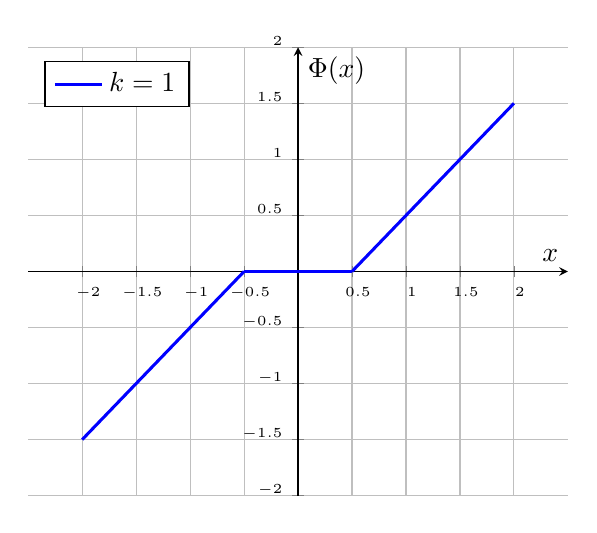
\begin{tikzpicture}
        \begin{axis} [
            xmin=-2.5, xmax=2.5, ymin=-2, ymax=2, grid=both,
            ylabel={$\Phi(x)$}, xlabel={$x$},
            xtick={-2,-1.5,...,2}, ytick={-2,-1.5,...,2},
            xticklabel style={font=\tiny, xshift=0.5ex},
            yticklabel style={font=\tiny, yshift=0.5ex},
            axis line style={->},
            axis x line=middle,
            axis y line=middle,
            legend pos=north west,
        ]
        \addplot+[mark=none, line width=1.1, color=blue, domain=-2:-0.5] {x+0.5};
        \addplot+[mark=none, line width=1.1, color=blue, domain=-0.5:0.5] {0};
        \addplot+[mark=none, line width=1.1, color=blue, domain=0.5:2] {x-0.5};
        \addlegendentry{$k=1$}
        \end{axis}
    \end{tikzpicture}

\end{document}
        \label{fig:chapter2:phi}
    }
    \subfloat[$\text{Play(x)}$]{
        \input{./tikz/play-by-phi}
        \label{fig:chapter2:play-by-phi}
    }
    \caption{(\myfigref{fig:chapter2:phi}) The graph of $\Phi(x)$. (\myfigref{fig:chapter2:play-by-phi}). There are three different dynamical progresses which initialize with different initial states.}
    \label{fig:chapter2:phi-and-play-by-phi}
\end{figure}

\begin{figure}
    \centering
    \subfloat[]{
    \raisebox{3.5ex} {
        \input{./tikz/nn-play-stepwise}
        \label{fig:chapter2:nn-play-stepwise}
    }
    }
    \hspace{40px}
    \subfloat[]{
        \documentclass{standalone}
\usepackage{tikz}
\usepackage{scalerel}

% \usetikzlibrary{positioning,chains,arrows}
\begin{document}
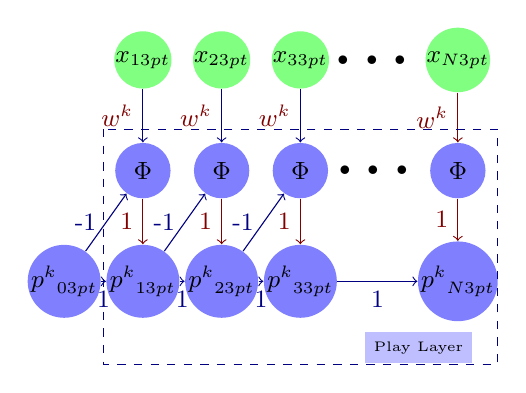
\begin{tikzpicture}[font=\small]
    % \draw (0.5,0.7) node [] {One Play};
    \tikzstyle{neuron}=[circle,fill=black!25,minimum size=20pt,inner sep=0pt];
    \tikzstyle{input neuron}=[neuron, fill=green!50];
    \tikzstyle{hidden neuron}=[neuron, fill=blue!50];
    \tikzstyle{activation neuron}=[neuron, fill=blue!50, rectangle, rounded corners=3pt, minimum size=13pt];
    \tikzstyle{play output neuron}=[neuron, fill=red!50, rectangle, rounded corners=3pt, minimum size=13pt];
    %% draw neurons
    \foreach \x in {1,2,3} {
        \node[input neuron] (x_\x) at (\x, 0) {$x_{\scaleto{\x}{3pt}}$};
        \node[hidden neuron] (phi_\x) at (\x,-40pt) {${\Phi}$};
    } 
    \foreach \x in {0,1,2,3}
        \node[hidden neuron] (p_\x) at (\x, -80pt) {${p^k}_{\scaleto{\x}{3pt}}$};

    \node[input neuron] (x_n) at (5,0) {$x_{\scaleto{N}{3pt}}$};
    \node[hidden neuron] (phi_n) at (5,-40pt) {$\Phi$};
    \node[hidden neuron] (p_n) at (5,-80pt) {${p^k}_{\scaleto{N}{3pt}}$};

    %% draw connections between nodes
    \foreach \x in {1,2,3} {
        \draw [->,color=blue!50!black] (x_\x) to node [left,color=red!50!black] {$w^k$} (phi_\x);
        \draw [->,color=red!50!black] (phi_\x) to node [left,color=red!50!black] {1} (p_\x);
    }
    \foreach \x / \y in {0/1,1/2,2/3} {
        \draw [->,color=blue!50!black] (p_\x) to node [left, color=blue!50!black] {-1} (phi_\y);
        \draw [->,color=blue!50!black] (p_\x) to node [below,color=blue!50!black] {1} (p_\y);
    }
    
    \draw [->,color=red!50!black] (x_n) to node [left,color=red!50!black] {$w^k$} (phi_n);
    \draw [->,color=red!50!black] (phi_n) to node [left,color=red!50!black] {1} (p_n);
    \draw [->,color=blue!50!black] (p_3) to node [below,color=blue!50!black] {1} (p_n);

    \path (x_3) -- (x_n) node[midway,scale=2,font=\bfseries] {\dots};
    \path (phi_3) -- (phi_n) node[midway,scale=2,font=\bfseries] {\dots};
    
    %% draw rectangle to include inputs/intermediate outputs
    \draw[dashed,thin,blue!50!black] (0.5,-25pt) rectangle (5.5, -110pt);
    \draw (4.5, -104pt) node [fill=blue!25!white] {\tiny Play Layer};

    % \draw[dashed,thin,green!50!black] (0.5,-12pt) rectangle (5.5, 12pt);
    % \node[] at (7, 0) {$X=[x_1,x_2,...,x_n]$};
    % \draw[dashed,thin,blue!50!black] (0.6,-68pt) rectangle (5.4, -92pt);
    % \node[] (op_output) at (2.8, -92pt) {};
    % \node[] at (7, -80pt) {$P=[p_1,p_2,...,p_n]$};
    

    % %% activation layer or non-linear layer
    % \begin{scope}[xshift=-13, yshift=-30]
    %     %% draw rectangle for non-linear layers
    %     \draw[dashed,thin,blue!50!black] (0,-105pt) rectangle (7, -136pt);
    %     \draw (6.05, -130pt) node [fill=blue!25!white] {\tiny Nonlinear Layer};
    %     %% draw rectangle for linear layers
    %     \draw[dashed,thin,red!50!black] (1.3,-142pt) rectangle (5.7,-171pt);
    %     \draw (4.9, -165pt) node [fill=red!25!white] {\tiny Linear Layer};

    %     % draw op output
    %     \foreach \s / \idx in {1/1,3/2} {
    %         \node[activation neuron] (activation_\idx) at (\s,-115pt) {\tiny $\tanh(\theta_{\scaleto{\idx}{2pt}}P+\theta_{\scaleto{\idx,0}{3pt}})$};
    %     }
    %     % draw non-linear node tanh(s)
    %     \node[activation neuron] (activation_s) at (6,-115pt) {\tiny $\tanh(\theta_{\scaleto{s}{2pt}}P+\theta_{\scaleto{s,0}{3pt}})$};
    %     % draw dots between two non-linear nodes
    %     \path (activation_2) -- (activation_s) node[midway,scale=2,font=\bfseries] {\dots};

    %     % draw play output
    %     \node[play output neuron] (play_output) at (3.5, -150pt) {\tiny $G^k=\sum_{s=1}^{S} \hat{\theta}_{\scaleto{s}{2pt}} \tanh(\theta_{\scaleto{s}{2pt}}P+\theta_{\scaleto{s,0}{3pt}}) + \hat{\theta}_{\scaleto{0}{2pt}}$};
        
    %     % draw connection between nonlinear layer and output layer, nonlinear layer and op_output layer
    %     \foreach \idx in {1,2} {
    %         \draw [->,color=blue!50!black] (op_output) to node [left,color=blue!50!black] {\tiny ${\theta}_{\scaleto{\idx}{2pt}}$} (activation_\idx);
    %         \draw [->,color=blue!50!black] (activation_\idx) to node [left,color=blue!50!black] {\tiny $\hat{\theta}_{\scaleto{\idx}{2pt}}$} (play_output);
    %     }
    %     \draw [->,color=blue!50!black] (op_output) to node [left,color=blue!50!black] {\tiny ${\theta}_{\scaleto{s}{2pt}}$} (activation_s); 
    %     \draw [->,color=blue!50!black] (activation_s) to node [left,color=blue!50!black] {\tiny $\hat{\theta}_{\scaleto{s}{2pt}}$} (play_output); 
    %     % draw connections \theta and \hat{\theta}
    % \end{scope}
\end{tikzpicture}
\end{document}

        \label{fig:chapter2:nn-play-rnn}
    }
    \caption{The neural network cell of \myformularef{eqn:chapter2:play-operator}. The arrows show how data flows in the cell, and the number of $w^k, 1, -1$ beside the arrow line is the weights of this cell. Note that only parameter $w_k$ is learnable in this network since parameters $-1, +1$ are fixed.}
    
\end{figure}
The dynamics of \myformularef{eqn:chapter2:play-operator} is shown in \myfigref{fig:chapter2:play-by-phi}, and it can be represented as a recurrent neural network (see \myfigref{fig:chapter2:nn-play-rnn}), using the elementary neural network cell displayed in \myfigref{fig:chapter2:nn-play-stepwise}.
% It can be represented as a RNN. Note that in such a form the network is not feed-forward.
% One can unfold it to make it feed-forward, see Fig. \ref{fig:chapter2:play-operator}

\begin{definition}\label{def:chapter2:play-networks}
If a network represents \myformularef{eqn:chapter2:play-operator}, we call this network a \textsl{play network}. If we apply nonlinear operators on this network to create a new network $\mathcal{P}$, we call $\mathcal{P}$ network generalized play network. 
\end{definition}
% \mytodo{add formula of generalized play network in appendix}

\begin{definition}\label{def:chapter2:m-unfolded}
If there are $N$ elements in the sequence $\{x_n\}$, we say the unfolded network is $N$-$unfolded$.
\end{definition}
For example, the network in \myfigref{fig:chapter2:nn-play-rnn} is N-unfolded.
% \mytodo{add picture/plot for 2-unfolded play network for example}

\section{Generalized Prandtl-Ishlinskii networks\label{sec:chapter2:pi-network}}
\begin{definition}
If a network $\mathcal{G}$ network is the linear combination of generalized play networks, we call this network generalized Prandtl-Ishlinskii network, or generalized PI network. If the length of input sequence is m, we call PI networks as $m$-unfolded PI networks.
\end{definition}

% \mytodo{add generalized play networks}

We consider a $\mathcal{G}$ network contains K $\mathcal{P}$ networks. Denote the initial states of $\mathcal{G}$ network 
% $p_0$. 
% and the output sequence of $k$th $\mathcal{P}$ network by
\begin{equation*}
    P_0 := (p^1_0, \ldots, p^K_0) \in \mathbb{R}^K
\end{equation*}

The generalized Prandtl-Ishlinskii (PI) operator maps
\begin{equation*}
    P_0, (x_1, x_2, \ldots) \mapsto (y_1, y_2, \ldots)
\end{equation*}
and is given by:
% \begin{equation*}
%     y_n = \sum_{k=1}^{K} \hat{\theta^{k}} p^k_n + \hat{\theta^{0}} = \sum_{k=1}^{K} \hat{\theta^{k}} \mathcal{P}(x_n, p^k_{n-1}, w^k) + \hat{\theta^{0}}
% \end{equation*}
\begin{equation}\label{eqn:chapter2:pi-contains-one-play}
    y_{n} = \sum_{k=1}^{K} \sum_{s=1}^{S} \hat{\theta}^{k}_{s} p^k_n + \hat{\theta}^{k}_{0} = \sum_{k=1}^{K} \sum_{s=1}^{S} \hat{\theta}^{k}_{s} \mathcal{P}(x_n, p^k_{n-1}, w^k) + \hat{\theta}^{k}_{0}, \quad n = 1,2,\ldots
\end{equation}
where $\hat{\theta}^{k}_{s},\hat{\theta}^{k}_{0}$ are parameters and $p^k_n$ are given by \myformularef{eqn:chapter2:play-operator}. It corresponds to a layer of plays or a \textit{PI network}, see \myfigref{fig:chapter1:nn-pi}.

% \section{Analysis of initial state $p_0$}

% Considering derivative of $p_n$ with respect to $p_0$, it's defined as
% \begin{equation}\label{eqn:chapter2:dynamic-p0}
% \frac{\partial p_{n}}{\partial p_0} = \prod_{i=1}^{n} \frac{\partial p_{i}}{\partial p_{i-1}} = \prod_{i=1}^{n} \left(1- \frac{\partial \Phi(u_i)}{\partial u_i}\Bigr|_{\substack{u_i=w x_{i} - p_{i-1}}}\right)
% \end{equation}

% where $\frac{\partial \Phi(u_i)}{\partial u_i}$ is given by
% \begin{equation}\label{eqn:chapter2:derviation-phi}
%   \begin{aligned}
%     \frac{\partial \Phi(u_i)}{\partial u_i} =
%     \begin{cases}
%       1, & p_{i-1} \in (-\infty, w x_{i}-0.5) \cup (w x_{i}+0.5, +\infty) \\
%       0, &  p_{i-1} \in (w x_{i}-0.5, w x_{i}+0.5)
%     \end{cases}
%   \end{aligned}
% \end{equation}

% From \myformularef{eqn:chapter2:derviation-phi} and \myformularef{eqn:chapter2:dynamic-p0}, 
% it's obvious that gradient on $p_0$ is trapped in vanishing situation if there exists a pair $(u_i, \Phi(u_i))$ where $u_i$ isn't on the horizontal part of $\Phi(u)$, see \myfigref{fig:chapter2:phi}. 


% If $n$ is sufficiently large,
% \begin{enumerate}
%     \item $k \in (0, 2]$, gradient on $p_0$ vanishes
%     \item $k \in (2, +\infty)$, gradient on $p_0$ explodes.
% \end{enumerate}

% \textbf{Solution.} We can split the input sequence into multiple batches and train the network on these smaller sequences to avoid gradient vanishing and exploding.

\mytodo{update parameters notation of architecture in chapter1}
\section{Training a PI network\label{sec:chapter2:training-pi-network}}
Assume we are given an input sequence $x_1, x_2, \ldots, x_N$ and an output sequence $y_1, y_2, \ldots, y_N$. We perform the following steps in cycle until convergence. 
\begin{enumerate}
\item Preparing initial states for the network: Fix a vector of initial states $P_0$ and all the weights (denoted by $W$, a collection of $w^k, \theta^{k}_{s}, \hat{\theta}^{k}_{s}, \theta^{k}_{s,0}, \hat{\theta}^{k}_{0}$). For each $k=1, \ldots, K$, we calculate recursively $p_{1}^{k}, p_{2}^{k}, \ldots, p_{N}^{k}$ by \myformularef{eqn:chapter2:play-operator}. We denote the corresponding states of the PI network by
  \begin{equation*}
    P_n = (p_{n}^{1}, \ldots, p_{n}^{K}), n = 1, \ldots, N.
  \end{equation*}
\item Preparing inputs for the $m$-unfolded network: We fix $m$ and group the input sequence into $m$-tuples:
  \begin{equation*}
    \mathbf{x_1} := (x_1, \ldots, x_m), \quad \mathbf{x_2} := (x_2, \ldots, x_{m+1}), \quad \ldots,
  \end{equation*}
  which gives $M := N-m$ tuples $\mathbf{x_1}, \ldots, \mathbf{x_M}$. Next we form a new set of inputs for the $m$-unfolded network, attaching the vectors of intermediate states:
  \begin{equation*}
    \mathbf{\tilde{x}_1} := (P_0, \mathbf{x_1}), \quad \mathbf{\tilde{x}_2} := (P_1, \mathbf{x_2}), \quad \ldots,
  \end{equation*}

\item Training the $m$-unfolded network: We use adam optimizer \citep{kingma2014adam} to train the $m$-unfolded \textit{PI network}
  \begin{equation*}
    \mathbb{R}^{K} \times \mathbb{R}^{m} \ni \mathbf{\tilde{x}} \mapsto F_{m}(\mathbf{\tilde{x}}) \in \mathbb{R}^m
  \end{equation*}
  with the inputs $\mathbf{\tilde{x}_1}, \ldots, \mathbf{\tilde{x}_M}$ and the true targets $\mathbf{y_1}, \ldots, \mathbf{y_M}$, where
  \begin{equation*}
    \begin{aligned}
      \mathbf{y_1} = (y_1, \ldots, y_m), \quad 
      \mathbf{y_2} = (y_2,\ldots, y_{m+1}), \quad 
      \ldots
    \end{aligned}
  \end{equation*}

\item Updating weights $W$.

% \begin{remark}\label{remark:chapter2:1}
%   Since $P_D(x)$ and $P_N(x)$ are not functions but operators, the monotone curves described in \ref{lemma:chapter3:reaction-to-price-change} are not defined only by the current value of $x$, but depend on its prehistory.
% \end{remark}

% $ At this step, we only update the weights $W$, but not the initial state $P_0$
% \item We update the initial state $P_0$:
%   \begin{equation*}
%     P_{0}^{new} := P_{0} - \nabla_{P_0} (F_m(P_0, \mathbf{x_1}) - \mathbf{q_1})^2
%   \end{equation*}
% \item Updating weights $W$
%   \begin{eqnarray*}
%     W^{new} := W - \nabla_{W} (F_m(P_0, \mathbf{x_1}) - \mathbf{q_1})^2 \\
%     % P_{0}^{new} := P_{0} - \nabla_{P_0}(F_m(P_0, \mathbf{x_1}) - \mathbf{q_1})^2
%   \end{eqnarray*}
% % \item \mytodo{TODO: Training state}
% % \item \todo{TODO: Training weights}

\end{enumerate}


\begin{remark}
For a hysteretical process trained by HNN, it will catch up with the trace after finite time steps even through the initial state is incorrect.
\mytodo{see evaluation results}
\end{remark}